--Description--

External services do not need to be unit tested since it is assumed that they are reliable. 

[The order of the implementation, and why that one!]


\subsection{Plan Definition}
The strategy adopted for this phase of the project is a \textbf{bottom-up}: it focuses on individual components of the system. 
Starts from the detailed part, then links these ones to others and form larger components, until the entire system is formed. In this way it is possible to make decisions about low-level utilities and then decide how there will be put together to create high-level construct.\\ \\
In some cases we follow a \textbf{top-down} approach: start from an overview without going into details; then go deeper into more details each step. Top-down approach is used when a component needs another one that manages data it needs, but the second one is not implemented yet. In this way can be created hypothetical data while developing the main functionality. As a result we need to be able to generate feasible \textbf{stubs} used to simulate the data that the system is going to manage both real or randomly, in order to cover more scenarios possibles.\\ \\
The description starts from server's component because it is the most complex part and the core one that organize the hole system.\\
During the implementation \textbf{drivers} are used to simulate components that are not implemented yet, or to generate possible request.\\
The components that retreive information from external system are implemented later because they had no particular "intelligence" in it, are used only to retreive information and do not need big test on them(here are created the stub, their data are not relly crucial for the current step of the implementation) 

\begin{enumerate}
    \item This is the first step of the implementation. \\Most of the component require the performance of the \textsl{Model} and \textsl{Data Manager} to retrieve information and use hem to reply a user’s request. For this reason they are going to be implemented and tested first. 
    \begin{figure}[H]
        \begin{center}
        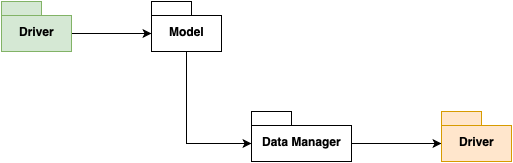
\includegraphics[width=1\textwidth]{implementation/step1.png}
        \caption{Implementation first step.}
        \label{fig:first step}
        \end{center}
    \end{figure}
    \item Then we start from the component that manage the access to the system. The reson is that this is a cructial phase of the application; it is how the user first approach the system and it's important that credential are well verified. The system must recognize the type of user to organize the application in the right way and reply with only the functionality permitted, so them affect the others components.\\ It is also a matter of privacy. 
    \begin{figure}[H]
        \begin{center}
        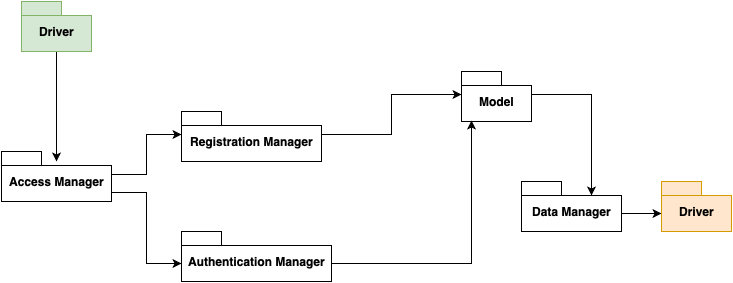
\includegraphics[width=1\textwidth]{implementation/step2.png}
        \caption{Implementation second step.}
        \label{fig:second step}
        \end{center}
    \end{figure}
    \item The main focus of the application is to help farmer with their production, so after the authentication the focus is on create the farm page with all the information that it requires. At first \textsl{Production Manager} to store or made visible the data about production and then \textsl{ViewInfo Manager} to create a first prototype of the farm page. Stub is used to fill the field in the page related to the weather.
    \begin{figure}[H]
        \begin{center}
        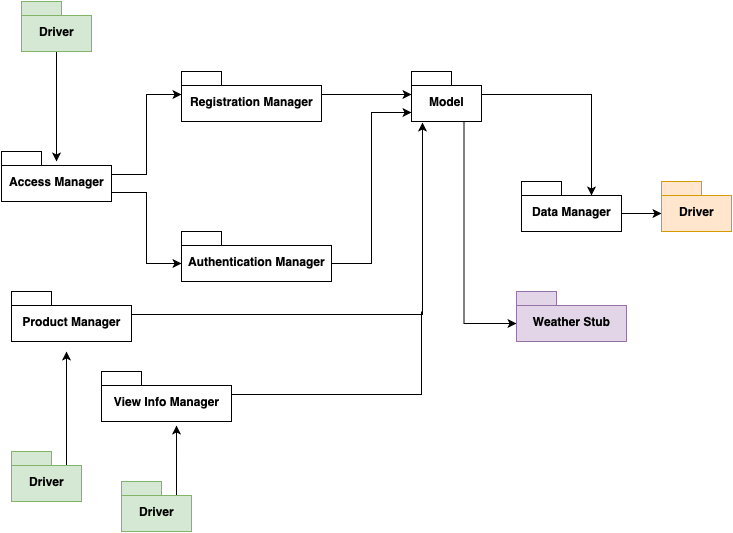
\includegraphics[width=1\textwidth]{implementation/step3.png}
        \caption{Implementation third step.}
        \label{fig:third step}
        \end{center}
    \end{figure}
    \item In this step the components related to the user ( \textsl{Web Servers} and \textsl{Web Application}) to create a real visualization and comuunication with these two part of the entire system, now that the main functionality can be used. A driver is used to create some possible request of the user and test the component yust integrated.
    \begin{figure}[H]
        \begin{center}
        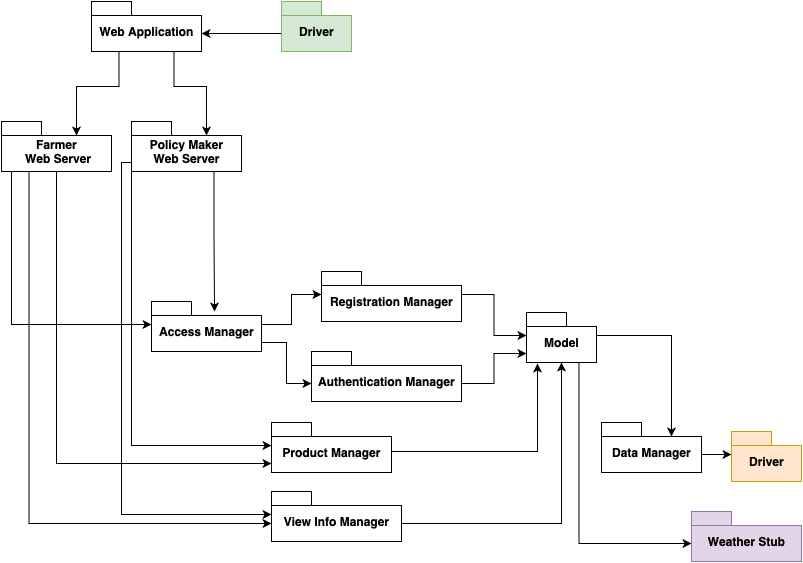
\includegraphics[width=1\textwidth]{implementation/step4.png}
        \caption{Implementation fourth step.}
        \label{fig:fourth step}
        \end{center}
    \end{figure}
    \item Now are added the components related to the other functionalities: retreive and send notification, with \textsl{Notification Manager} because farmer and policy maker ware "implemented" before, so it is possible to them to kind of comunicate through this component. The second functionality is to make able the farmers to comunicate to each other via forum, so the \textsl{Forum Manager} is created. The third is the visualization of the map so is integrated a stub just to test ifthge other components fill it with the right data. At this point all the pages can be created.
    \begin{figure}[H]
        \begin{center}
        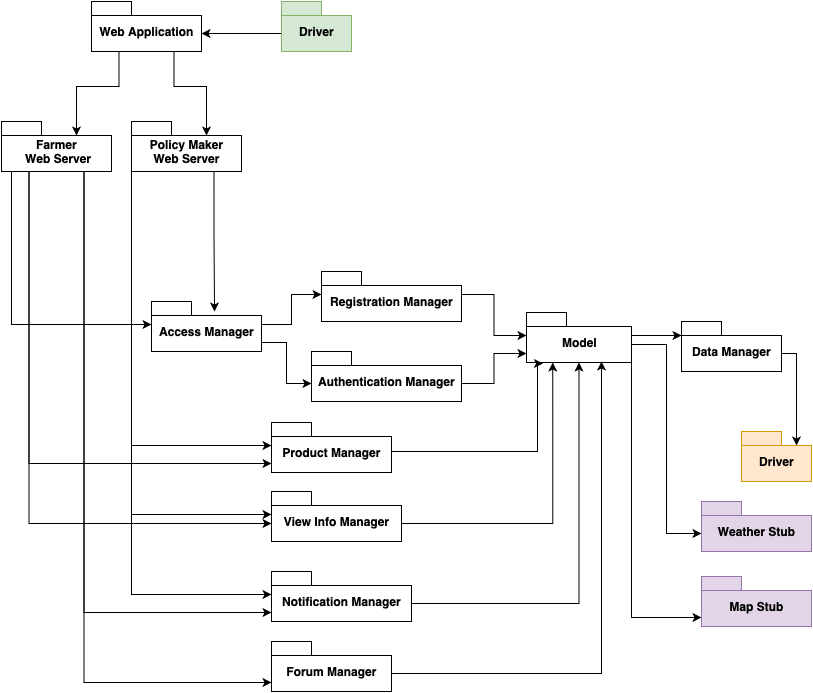
\includegraphics[width=1\textwidth]{implementation/step5.png}
        \caption{Implementation fifth step.}
        \label{fig:fifth step}
        \end{center}
    \end{figure}
    \item At least we integrate the components that comunicate with the external systems and retreive the real data, in the pages now are all "real" information. Now it is the implementation of the hole system.
    \begin{figure}[H]
        \begin{center}
        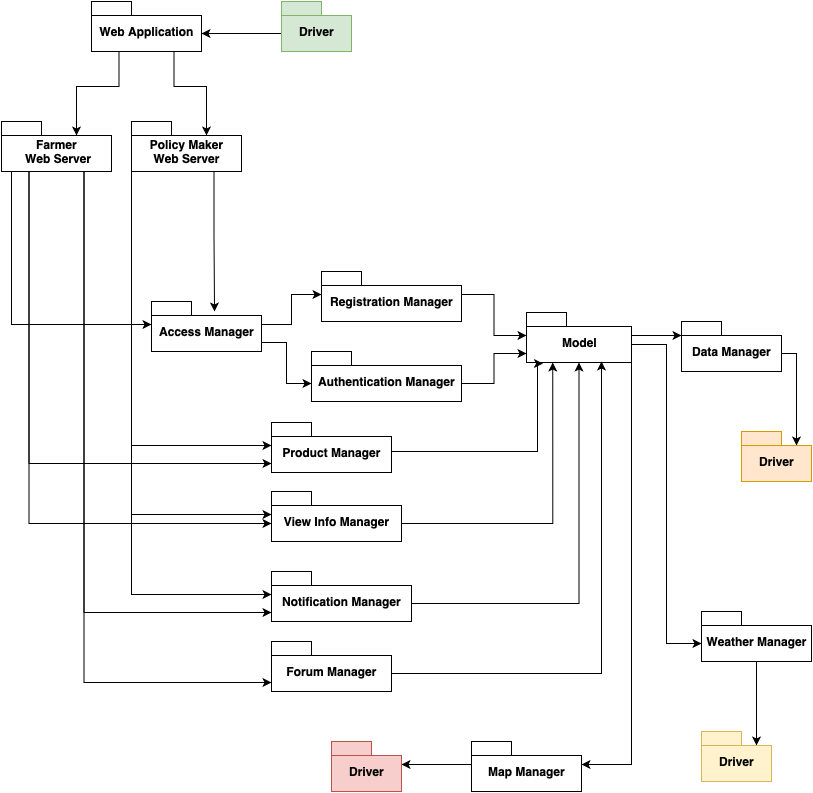
\includegraphics[width=1\textwidth]{implementation/step6.png}
        \caption{Implementation sixth step.}
        \label{fig:sixth step}
        \end{center}
    \end{figure}
\end{enumerate}